
%=========================================================
\section{Módulos del sistema}

El sistema se encuentra organizado en módulos, con la finalidad de agrupar y administrar de mejor manera los requerimientos funcionales del sistema. Dividir el sistema en módulos permite visualizar e identificar rápidamente aquellos aspectos funcionales que pueden tratarse conjuntamente. La figura \ref{fig:modulos} muestra los módulos propuestos para el sistema.

\begin{figure}[h!]
	\begin{center}
		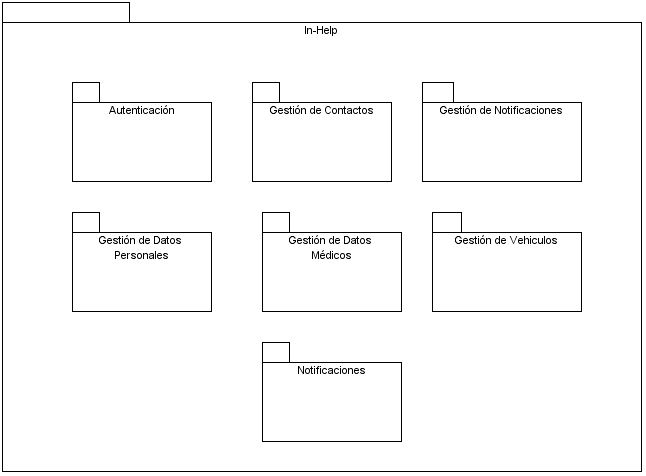
\includegraphics[scale=0.4]{ModeloComportamiento/imagenes/modulosSistema.png}
		\caption{Módulos del sistema.}
		\label{fig:modulos}
	\end{center}
\end{figure}

%A continuación se describen de manera general cada uno de los módulos:
%
%\begin{itemize}
%	\item {\bf Aplicación Móvil:} Agrupa los casos de uso que tienen que ver con el proceso de lectura de los signos vitales medidos por el sistema embebido, a través de los cuáles, el usuario puede agregar, consultar, editar y eliminar información del paciente que utilice el sistema, así como visualizar el historial del mediciones realizadas.
%	
%	\item {\bf Sistema Embebido:} 
%		
%\end{itemize}
%\pagebreak